\documentclass[en]{snu-ece-bsc-thesis}

% --- Math / units / graphics ----------------------------------------
\usepackage{siunitx}
\usepackage{booktabs}
\usepackage{multirow}
\usepackage{algorithm}
\usepackage{algpseudocode}

\usepackage{tikz}
\usetikzlibrary{positioning, fit, arrows.meta, calc, decorations.pathreplacing}

% --- Bibliography ---------------------------------------------------
\addbibresource{bib.bib}

% --- hyperref MUST be loaded last -----------------------------------
\usepackage[pdfusetitle]{hyperref}

% =====================================================================
% Document metadata
% =====================================================================
\title{DCT-Page: Frequency-Domain Page Proxies for\\Sparse KV Decoding}
\author{김윤곤}
\advisor{김재준}
\date{2026년 12월}                    % TODO: confirm submission month
\approvaldate{2026년 12월}             % TODO: confirm approval month

\koreankeywords{장문맥 언어모델, 희소 어텐션, KV 캐시,
                이산 코사인 변환, 페이지 어텐션}
\englishkeywords{Long-context Language Model, Sparse Attention, KV Cache,
                 Discrete Cosine Transform, Page Attention}

% =====================================================================
\begin{document}
\maketitle

% --- Front matter ---------------------------------------------------
\pagenumbering{roman}

\begin{abstract}
% TODO: write after the rest of the thesis is drafted.
% Target length: ~250-300 words.
% Cover (1) problem, (2) insight, (3) method, (4) headline results, (5) impact.
\end{abstract}

\tableofcontents
\listoftables
\listoffigures

% --- Body -----------------------------------------------------------
\pagenumbering{arabic}

\chapter{Introduction}\label{chap:introduction}

% Target length: ~3 pages.
% Open with the KV-cache decode bottleneck, name the gap in prior sparse-
% attention methods, state the low-frequency insight, summarize 3-4
% contributions, then list the thesis organization.


\section{Motivation}\label{sec:motivation}
% TODO


\section{Key Insight: Attention Keys are Low-Frequency}\label{sec:intro-insight}
% TODO: foreshadow the central observation. 1-2 paragraphs + forward
% reference to Figure in Chapter 3.


\section{Contributions}\label{sec:contributions}
% TODO: 3-4 bullets, copied from poster and tightened.
%   1. Training-free DCT-lowpass-IDCT page scoring (drop-in monkey-patch).
%   2. Fused Triton kernels turning sparsity into measured throughput.
%   3. Comprehensive evaluation across RULER / LongBench v1 / v2 with
%      4 sparse-attention baselines.
%   4. Attention-mass-recall analysis pinning down why DCT-Page works.


\section{Thesis Organization}\label{sec:organization}
% TODO: one short paragraph mapping chapters to their roles.

\chapter{Background and Related Work}\label{chap:background}


% =====================================================================
\section{Autoregressive Decoding and the KV-Cache Bottleneck}\label{sec:kv-bottleneck}
% =====================================================================

Decoder transformers~\cite{vaswani2017attention} generate text
autoregressively: at decode step $t$, the model conditions on every
previously emitted token and produces a single new token.  The
attention mechanism at each layer computes, for the current
query~$q_t \in \mathbb{R}^{d}$ and the cumulative keys
$K_{\le t} \in \mathbb{R}^{t \times d}$ and values
$V_{\le t} \in \mathbb{R}^{t \times d}$,
\begin{equation}\label{eq:attn}
  \mathrm{Attn}(q_t, K_{\le t}, V_{\le t})
  \;=\;
  \mathrm{softmax}\!\bigl(q_t K_{\le t}^{\top} / \sqrt{d}\bigr)\,V_{\le t}.
\end{equation}
To avoid recomputing the past keys and values at every step, modern
inference runtimes maintain a \emph{KV cache} that grows by one row
per decode step.  Each step then performs an inner product between
$q_t$ and the entire cached $K_{\le t}$, followed by a softmax-weighted
read of $V_{\le t}$.

The cost of Eq.~\eqref{eq:attn} per decode step is dominated by the
memory traffic of reading the cache.  At context length $L$, the per-step
attention reads $O(L \cdot d)$ entries of $K$ and $V$ from GPU global
memory, and the arithmetic intensity of the operation (a single small
matrix--vector product per head) is far below the compute-to-memory
ratio of modern accelerators.  As a result, decode latency scales
approximately linearly with $L$ and is bottlenecked by HBM bandwidth
rather than by FLOPs.  At $L = 128$K with an 8B-parameter model in
\texttt{bfloat16}, the KV cache alone can occupy more than half of the
device memory budget, and the per-step attention can take longer than
all other layer operations combined.

Two structural observations sit behind every sparse-attention
proposal of the past two years.  First, even at long context the
dense softmax in Eq.~\eqref{eq:attn} concentrates most of its mass
on a small subset of past tokens; the rest contributes negligible
energy and could in principle be skipped without changing the output.
Second, prefill --- the one-pass attention over the prompt that
populates the cache --- is compute-bound rather than memory-bound.
Concretely, prefill on an $L$-token prompt computes a $Q[L \times d]
\cdot K^{\top}[d \times L]$ matrix--matrix product (arithmetic
intensity $O(L)$ FLOP per byte loaded), whereas decode computes a
$q[1 \times d] \cdot K^{\top}[d \times L]$ matrix--vector product
(arithmetic intensity $O(1)$, independent of $L$).  For any $L$ on
the order of a thousand or more, prefill is therefore in the
compute-bound regime and modifying it offers little speedup, while
decode is squarely memory-bound.  Sparse-attention
systems --- DCT-Page included --- therefore typically leave prefill
unchanged and intervene only at decode time, replacing the full read
of $K_{\le t}, V_{\le t}$ with some compressed or filtered surrogate.


% =====================================================================
\section{Sparse and Compressed KV Attention}\label{sec:related-sparse}
% =====================================================================

The methods DCT-Page is compared against differ along two structural
axes: (i) how they \emph{group} the KV cache into selectable units
--- fixed-size pages or learned clusters --- and (ii) how they
\emph{score} each unit against the current query.  The first three
methods below share the page-based paradigm with DCT-Page; Multipole
sits in the cluster-based paradigm and is discussed last.

\subsection{Quest}\label{sec:rel-quest}

Quest~\cite{tang2024quest} partitions the KV cache into fixed-size
pages and, for each page, stores a pair of per-channel summary
statistics: the elementwise minimum and maximum of the keys inside
the page.  At decode time the query is scored against every page by an
\emph{approximate-max inner product}.  For each channel
$c \in \{1, \dots, d\}$, the per-channel contribution is taken to be
the larger of $q[c] \cdot \min_p[c]$ and $q[c] \cdot \max_p[c]$ ---
since the true key value $k[c]$ for any token inside the page lies in
$[\min_p[c], \max_p[c]]$, this is a tight upper bound on
$q[c] \cdot k[c]$ --- achievable when some token in the page attains
the channel extreme --- and selecting between $\min_p[c]$ and
$\max_p[c]$ requires only the per-channel sign of $q[c]$ ($\max_p[c]$
if $q[c] \ge 0$, $\min_p[c]$ otherwise).
The page score is the sum of these per-channel upper bounds across
the $d$ channels, which is itself an upper bound on
$\max_{k \in \text{page}} q^{\top} k$.  This bound is cheap (two
scalars per channel) and position-agnostic.  Quest then attends to the
top-$k$ pages by this score and ignores the rest.

The per-page metadata is small --- two scalars per channel rather
than a learned proxy --- and the kernel cost of scoring is low, which
makes Quest fast at moderate context length.  However, the min/max
abstraction discards \emph{intra-page} structure entirely: it cannot
distinguish a page in which a few channels happen to span a wide
range from a page in which one specific token has a large inner
product with the query.  Section~\ref{sec:quest-collapse} returns to
this point empirically.

\subsection{SeerAttention-R}\label{sec:rel-seer}

SeerAttention-R~\cite{gao2025seerattention} adds a small learned
\emph{gate} to each decoder layer that, at decode time, predicts
per-block importance scores from the current query.  The gate is
trained on long-context data with a supervision signal derived from
the dense attention distribution, so that its block scores correlate
with the softmax mass that the dense model would have placed on each
block.  At inference, the gates are evaluated at every layer and the
top-$k$ blocks are kept under a fixed token budget.

The learned-gate approach can be very accurate at a given budget
because it is explicitly optimized for the selection task, but it
imposes two practical constraints.  First, a model-specific
checkpoint must be released for every base model; in our experiments
we use the Qwen3-family gates released by the authors, since no
equivalent Llama-3 gates are available, and SeerAttention-R is
therefore reported on Qwen3-8B only.  Second, the gate adds a small
but non-zero per-layer parameter count and forward-time cost, which
slightly reduces its ceiling on raw decode throughput.

\subsection{InfLLM}\label{sec:rel-infllm}

InfLLM~\cite{xiao2024infllm} approaches long-context decoding from a
retrieval perspective.  The past KV cache is broken into blocks; each
block is summarized by a small set of \emph{representative tokens}
chosen by an upstream-defined importance heuristic; and at decode
time the current query is matched against every block's
representatives to produce a relevance score.  InfLLM additionally
keeps an initial sink region (the first $n_\text{init}$ tokens) and a
local sliding window, attending in full to both regardless of the
retrieval result.  Only the top-ranked blocks outside the sink and
local zones are read at full precision.

The retrieval framing makes InfLLM agnostic to context length in
principle, but it pays for this flexibility in implementation
complexity: the block representatives must be selected and indexed
carefully, and the published code path currently targets the Llama-3
family only.  We accordingly report InfLLM on Llama-3.1-8B-Instruct
alone.

\subsection{Multipole Attention}\label{sec:rel-multipole}

Multipole Attention~\cite{hooper2025multipole} departs from the
fixed-page paradigm and instead clusters keys with hierarchical
$k$-means.  At decode time the query attends through cluster
centroids: each cluster contributes a single representative key/value
pair, and clusters whose centroids score highly are then expanded to
their constituent keys for the final attention.  This is the
attention analogue of the fast-multipole-method approximation used in
$n$-body simulation.

Cluster-based selection has two strengths and one structural
weakness.  Its strengths are that the cluster representatives carry
within-page structure (a centroid is a positionless but
distribution-aware summary) and that the hierarchical structure
allows variable-width effective receptive fields per layer.
Empirically this yields the highest long-context accuracy among the
methods we evaluate (Section~\ref{sec:results-multipole}).  Its
weakness is that clusters are \emph{data-dependent and recomputed
during generation}: the centroids must be re-estimated as the KV
cache grows, and the keys belonging to a selected cluster are
scattered (non-contiguous) in memory.  The per-step computation
therefore has an irregular memory-access pattern that does not
amortize across decode steps the way a fixed page layout does, and
the decode-time wall clock is substantially slower than the
page-based methods at the same selected-token budget.
This is the source of the accuracy--throughput Pareto trade-off that
Section~\ref{sec:results-multipole} reports in detail.


% =====================================================================
\section{Frequency-Domain Signal Compression}\label{sec:related-freq}
% =====================================================================

The DCT proxy of Section~\ref{sec:proxy} is a low-rank linear
projection of a key sequence onto its leading discrete-cosine
coefficients.  We collect here the small set of background facts that
make this projection well-behaved for our application.

\paragraph{Discrete cosine transform.}
The type-II DCT used in Eq.~\eqref{eq:dct} is an orthonormal linear
transform that asymptotically diagonalizes the second-order
autocorrelation matrix of a stationary Markov-1 signal --- this is
the classical motivation for its dominance in image and audio
codecs (e.g.\ JPEG)~\cite{rao1990dct}.  Orthonormality means that energy is
preserved under DCT, and Parseval's theorem applies coefficient by
coefficient: discarding the higher-frequency bins reduces the
sequence's $\ell_2$ norm by exactly the energy of those bins.
Whether the resulting low-rank reconstruction is a good summary of
the original signal therefore reduces to whether the signal's energy
is in fact concentrated in the leading bins, which is the empirical
question raised in Section~\ref{sec:insight}.

\paragraph{Lowpass-IDCT as a linear projection.}
Concatenating a length-$P$ DCT, a truncation that keeps the first $C$
coefficients, and a length-$C$ inverse DCT yields a single
$C \times P$ matrix that can be precomputed once and applied as a
small dense matrix multiply at runtime.  This is the operator
$M \in \mathbb{R}^{C \times P}$ of Eq.~\eqref{eq:proxy}.  All of the
mass-recall and accuracy results in Chapter~\ref{chap:results} use
this single fixed $M$; nothing about the proxy is learned.

\paragraph{Concurrent frequency-domain work.}
The closest contemporary system is
FreqKV~\cite{kai2026freqkv}, which uses a DCT-based representation
to compress the KV cache for context-window extension rather than
for sparse decoding.  FreqKV operates in the prefill stage and
modifies the cache layout itself, whereas DCT-Page leaves the cache
unchanged and uses DCT only as a scoring proxy during decode.  The
two systems are complementary --- one could in principle combine
FreqKV's frequency-domain prefill compression with DCT-Page's
frequency-domain decode-time scoring --- but in this thesis we
restrict attention to the decode-time use of DCT.

\chapter{Method: DCT-Page}\label{chap:method}

DCT-Page modifies only the \emph{decode} path of attention.
During prefill the model runs unchanged, producing an ordinary
key--value (KV) cache.  At decode time the cache is reinterpreted as a
sequence of fixed-size pages, each page is summarized by a short
low-frequency proxy, and the query attends to a constant-size subset:
the sink, the top-$k$ pages by proxy score, and a small recent window.
The remaining pages are skipped entirely.
This chapter describes the layout, the proxy, the selection rule, and
the fused kernels that turn the resulting sparsity into measured
throughput.


\section{Decode-Time Page Layout}\label{sec:layout}

Let $L$ denote the current KV-cache length and $P$ the page size
(default $P{=}32$).  Let $S$ and $R$ be the number of sink and full
recent pages, respectively.  The cache is partitioned as
\begin{equation}\label{eq:layout}
  \underbrace{[\,0,\; SP\,)}_{\text{sink}}\;\Big\|\;
  \underbrace{[\,SP,\; SP{+}NP\,)}_{\text{middle pages}}\;\Big\|\;
  \underbrace{[\,SP{+}NP,\; L\,)}_{\text{recent}},
\end{equation}
where
\begin{equation}\label{eq:num-pages}
  N \;=\; \left\lfloor \frac{L - SP - RP}{P} \right\rfloor
\end{equation}
is the number of \emph{middle} pages, i.e.\ the pageable region from
which DCT-Page selects.
The recent zone consists of $R$ full pages plus a partial \emph{open}
page that absorbs the most recent $0,\dots,P{-}1$ tokens; the open page
is always attended in full.
Figure~\ref{fig:layout} shows the layout for $S{=}1,\ R{=}4$, the
defaults used throughout this thesis.

\begin{figure}[ht]
  \centering
  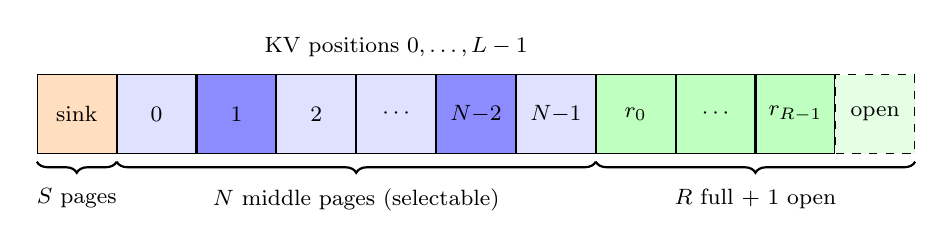
\begin{tikzpicture}[
    page/.style={draw, rectangle, minimum height=10mm, minimum width=10mm,
                 inner sep=0pt, font=\footnotesize},
    sink/.style ={page, fill=orange!25},
    mid/.style  ={page, fill=blue!12},
    selmid/.style={page, fill=blue!45},
    rec/.style  ={page, fill=green!25},
    open/.style ={page, fill=green!10, dashed},
    brace/.style={decoration={brace, amplitude=4pt, mirror}, decorate, thick},
    lbl/.style={font=\footnotesize}
  ]
    % Cells
    \node[sink]                     (s0)  at (0,0)        {$\mathrm{sink}$};
    \node[mid,    right=0mm of s0]  (m0)                  {$0$};
    \node[selmid, right=0mm of m0]  (m1)                  {$1$};
    \node[mid,    right=0mm of m1]  (m2)                  {$2$};
    \node[mid,    right=0mm of m2]  (m3)                  {$\cdots$};
    \node[selmid, right=0mm of m3]  (m4)                  {$N{-}2$};
    \node[mid,    right=0mm of m4]  (m5)                  {$N{-}1$};
    \node[rec,    right=0mm of m5]  (r0)                  {$r_0$};
    \node[rec,    right=0mm of r0]  (r1)                  {$\cdots$};
    \node[rec,    right=0mm of r1]  (r2)                  {$r_{R-1}$};
    \node[open,   right=0mm of r2]  (op)                  {open};

    % Braces and labels (mirror=true so the central peak points up toward
    % the cells; the labels sit below).
    \draw[brace] ($(s0.south west)+(0,-1mm)$)
              -- ($(s0.south east)+(0,-1mm)$)
       node[midway, below=6pt, lbl] {$S$ pages};
    \draw[brace] ($(m0.south west)+(0,-1mm)$)
              -- ($(m5.south east)+(0,-1mm)$)
       node[midway, below=6pt, lbl] {$N$ middle pages (selectable)};
    \draw[brace] ($(r0.south west)+(0,-1mm)$)
              -- ($(op.south east)+(0,-1mm)$)
       node[midway, below=6pt, lbl] {$R$ full + 1 open};

    % Top label
    \node[above=1mm of m3, lbl] {$\text{KV positions } 0,\dots,L-1$};
  \end{tikzpicture}
  \caption[Decode-time KV page layout used by DCT-Page.]
  {Decode-time KV layout. The sink and recent zones are always
  attended; only the $N$ middle pages enter the top-$k$ selection.
  Darker blue cells indicate two example selected pages.}
  \label{fig:layout}
\end{figure}

\paragraph{Sink and recent zones.}
The sink absorbs the initial-token attention sinks observed in
autoregressive decoder transformers and is kept verbatim to preserve
position-aware behaviors learned during pretraining.
The recent window protects the most local context, which dominates the
output for generation tasks and is cheap to keep at full resolution.

\paragraph{Page granularity.}
The page size is the fundamental trade-off knob.  A smaller $P$ gives
finer selection but raises bookkeeping cost (more pages, more scores,
more top-$k$ work).  A larger $P$ amortizes overhead but loses
selectivity within the page.  We use $P{=}32$ throughout, which is
also the granularity at which contemporary sparse-attention systems
operate (Quest, SeerAttention-R, Multipole).

\paragraph{Fallback below short context.}
When $L$ is short, the savings from sparsification are dominated by
the bookkeeping overhead of scoring and assembly.  DCT-Page therefore
falls back to standard dense decode attention when
$L < L_\text{min}$, with $L_\text{min}{=}8192$ tokens by default.


\section{Key Insight: Low-Frequency Structure of Attention Keys}\label{sec:insight}

The starting point for the rest of this chapter is a single empirical
observation about decoder-transformer key vectors: viewed as a signal
along the sequence axis, they are overwhelmingly low-frequency.

Concretely, take a page of $P{=}32$ consecutive keys
$K_p \in \mathbb{R}^{P \times d}$ from a single (batch, layer, head)
triple and apply the orthonormal type-II discrete cosine transform
along the sequence axis,
\begin{equation}\label{eq:dct}
  \hat K_p[m, c] \;=\;
  \sqrt{\tfrac{2}{P}}\, \alpha_m \sum_{n=0}^{P-1}
  K_p[n, c]\,
  \cos\!\left(\tfrac{\pi (2n{+}1) m}{2P}\right),
  \quad m = 0,\dots,P{-}1,
\end{equation}
with $\alpha_0 = 1/\sqrt{2}$ and $\alpha_m = 1$ for $m \ge 1$.
Here $\hat K_p \in \mathbb{R}^{P \times d}$ is the frequency-domain
representation of the page: row index $m$ runs over DCT bins from low
($m{=}0$, the DC term) to high frequency, and each column $c$ holds
the spectrum of one of the $d$ feature channels.
By Parseval's theorem (DCT is orthonormal), the total energy of $K_p$
equals the sum of squared coefficients $\sum_m \|\hat K_p[m, :]\|^2$.
On a RULER NIAH-MultiKey~3 trace at 32K context with
Llama-3.1-8B-Instruct, the first four DCT bins ($m = 0, 1, 2, 3$)
capture, on average, $\approx 85\%$ of the total per-page key energy
across layers, and the first eight bins reach $\approx 90\%$; the
remaining high-frequency tail contributes negligibly
(Figure~\ref{fig:dct-energy}).

\begin{figure}[ht]
  \centering
  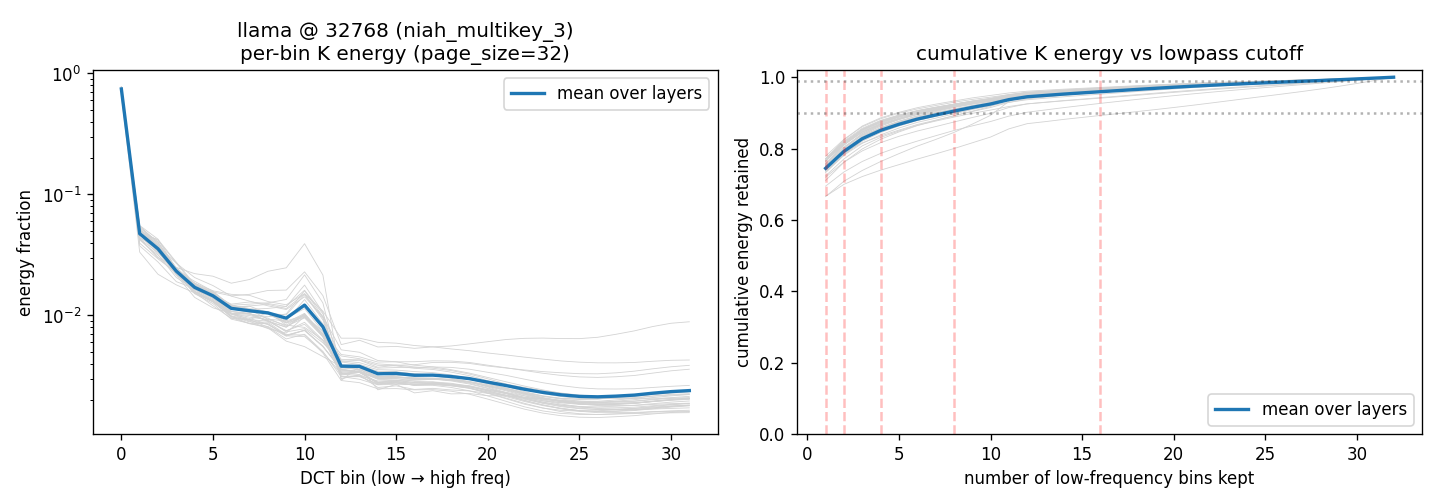
\includegraphics[width=0.95\textwidth]{figures/energy_curve.png}
  \caption[Per-bin DCT energy of KV-cache key pages.]
  {Per-bin DCT energy and cumulative energy of decoder-transformer
  key pages on Llama-3.1-8B-Instruct, page size $P{=}32$, RULER
  NIAH-MultiKey~3 at 32K context. Left: per-bin energy fraction;
  each thin grey line is a single transformer layer, the thick blue
  line is the across-layer mean. The spectrum is strongly low-pass.
  Right: cumulative fraction of energy retained as a function of the
  lowpass cutoff; the first four bins already cover $\approx 85\%$
  of the per-page energy and eight bins cover $\approx 90\%$.}
  \label{fig:dct-energy}
\end{figure}

This concentration has a direct consequence for sparse attention.
The attention score that determines whether page $p$ should be
selected for a query $q$ is the inner product
$q^\top K_p[n, \cdot]$ for some token $n$ in the page.  If $K_p$
itself lives in a low-rank low-frequency subspace, then a DCT-lowpass
reconstruction of $K_p$ should be a near-lossless proxy for the
selection score, even after collapsing $P$ tokens into a handful of
representative tokens.  The next section formalizes this proxy and
quantifies how well it routes queries to the right page.


\section{DCT-lowpass-IDCT Page Proxy}\label{sec:proxy}

Section~\ref{sec:insight} established that a page of keys
$K_p \in \mathbb{R}^{P \times d}$ is concentrated in its leading DCT
bins.  DCT-Page exploits this by replacing each page with a much
shorter sequence that retains only those bins.

Fix a target proxy length $C$ with $1 \le C \le P$
(``compression ratio'' $C/P$).  Let
$F_P \in \mathbb{R}^{P \times P}$ be the orthonormal DCT-II matrix
from Eq.~\eqref{eq:dct}, let $F_C \in \mathbb{R}^{C \times C}$ be the
same construction with $P$ replaced by $C$, and let
$E_C = [\,I_C \;\mid\; 0\,] \in \mathbb{R}^{C \times P}$ select the
first $C$ coordinates.  The DCT-lowpass-IDCT page proxy is
\begin{equation}\label{eq:proxy}
  K_p^{\text{proxy}} \;=\; M\,K_p
  \quad\text{with}\quad
  M \;=\; \sqrt{\tfrac{C}{P}}\;
          F_C^{\top}\, E_C\, F_P
          \;\in\; \mathbb{R}^{C \times P},
\end{equation}
i.e.\ apply the length-$P$ DCT, keep the leading $C$ coefficients,
apply the length-$C$ IDCT, and rescale by $\sqrt{C/P}$ so that the
$C$-token proxy matches the per-token energy density of the original
$P$-token page.  Crucially $M$ depends only on $(P, C)$, so it is
computed once at start-up and cached as a single $C \times P$ matrix;
at runtime, proxy construction is a single batched matrix multiply.

\paragraph{Compression knob.}
The proxy length $C$ trades selection fidelity against proxy-cache
size and per-step compression cost.  At $C{=}1$ the entire page
collapses to a single token, which is fast and minimizes memory but
discards the higher-frequency structure that distinguishes pages from
one another.  At $C{=}4$ the proxy keeps the four energetic bins
identified in Figure~\ref{fig:dct-energy}, capturing $\approx 85\%$
of the per-page key energy while still compressing the cache by $8\times$.
The main configuration in this thesis uses $C{=}4$ (i.e.\ a
$\text{compress\_ratio}$ of $1/8 = 0.125$); Section~\ref{sec:ablations}
reports the sweep over $C \in \{1, 2, 4, 8\}$ that justifies this
choice.

\paragraph{Incremental update during decode.}
A decode step appends one token to the KV cache.  Until the currently
open page accumulates a full $P$ tokens it lives in the recent zone
and is attended in full; only when it closes does it become a new
middle page and require its proxy to be computed.  Consequently at
most one new page closes per decode step, and the proxy cache is
updated as
\begin{equation}\label{eq:incremental-update}
  K_{\text{new}}^{\text{proxy}}
  \;=\;
  M\,K_{\text{new}},
  \qquad
  M \in \mathbb{R}^{C \times P},\;
  K_{\text{new}} \in \mathbb{R}^{P \times d}.
\end{equation}
This is a single matrix multiply per (batch, kv-head) tuple, costing
$O(P \cdot C \cdot d)$ scalar multiplications.  The cost is paid
\emph{only when a page closes}, i.e.\ once every $P$ decode steps, so
amortized per-step compression work is $O(C \cdot d)$.

After $N$ middle pages have accumulated the proxy cache occupies
$O(N \cdot C \cdot d)$ entries per (batch, kv-head).  Both the cache
size and the per-page compression cost depend only on the number of
\emph{closed} middle pages and the page size $P$, not on the total
context length $L$; the proxy machinery therefore imposes no extra
context-length scaling on top of the unavoidable $O(L)$ KV cache
itself.


\section{Scoring and Top-k Selection}\label{sec:scoring}

The proxy cache from Section~\ref{sec:proxy} feeds the page-scoring
step.  Let
$Q \in \mathbb{R}^{H_q \times d}$ be the decode query (one token,
$H_q$ query heads) and let the model use grouped-query attention
(GQA) with $H_k$ key-value heads and $G = H_q / H_k$ query heads per
group.  Index query heads by $(h, j)$ where $h$ is the KV head and
$j \in \{0, \dots, G{-}1\}$ is the position within the group.

\paragraph{Per-page score.}
For page $p$ with proxy
$K_p^{\text{proxy}} \in \mathbb{R}^{C \times d}$,
form the scaled inner products
\begin{equation}\label{eq:innerprod}
  g_{h,j,p,c} \;=\;
  \frac{1}{\sqrt{d}}\,
  Q_{h,j}^{\top}\,K_p^{\text{proxy}}[c, :],
  \qquad c = 0, \dots, C{-}1,
\end{equation}
and reduce over the $C$ proxy tokens with a
\emph{proxy-token aggregator} $\rho \in \{\max, \mathrm{mean}\}$ and
over the $G$ query heads in the GQA group with a
\emph{GQA-group aggregator} $\gamma \in \{\max, \mathrm{mean}\}$:
\begin{equation}\label{eq:score}
  S_{h,p}
  \;=\;
  \gamma_{j=0,\dots,G-1}
  \Bigl(\,
    \rho_{c=0,\dots,C-1}\, g_{h,j,p,c}
  \,\Bigr).
\end{equation}
$S_{h,p}$ is a single scalar measuring how relevant page $p$ is to
kv-head $h$'s decode query.  The default configuration is
$\rho = \max$ and $\gamma = \max$, which matches a hottest-token /
hottest-head heuristic: page $p$ scores high if \emph{any} query head
in the group has a large inner product with \emph{any} of its proxy
tokens.  Section~\ref{sec:ablations} reports sensitivity to these
choices.

\paragraph{Top-$k$ selection.}
Let $\mathcal{T}_h \subseteq \{0, \dots, N{+}R\}$ denote the set of
\emph{page indices} that kv-head $h$ will attend to during the current
decode step.  DCT-Page constructs $\mathcal{T}_h$ as the union of
three pieces:
\begin{equation}\label{eq:select}
  \mathcal{T}_h
  \;=\;
  \underbrace{\{0, \dots, S{-}1\}}_{\text{sink pages}}
  \;\cup\;
  \mathrm{TopK}_{k}\!\bigl(S_{h,\cdot}\bigr)
  \;\cup\;
  \underbrace{\{N, \dots, N{+}R\}}_{\text{recent + open pages}},
\end{equation}
where $\mathrm{TopK}_k$ returns the $k$ middle-page indices with the
largest scores $S_{h,p}$.  Note that the top-$k$ set is selected
\emph{per kv-head}, so different heads in the same layer may pick
different pages.  The decode then performs ordinary
scaled-dot-product attention against the keys and values gathered from
$\mathcal{T}_h$; the remaining $N - k$ middle pages contribute
\emph{nothing} to the output.

To match comparable sparse-attention baselines fairly, we report
budgets as the total number of \emph{fixed-size} pages attended per
step, denoted $B$, defined as
\begin{equation}\label{eq:budget}
  B \;=\; S + k + R,
\end{equation}
the sum of the sink, selected-middle, and full-recent contributions.
The selection rule of Eq.~\eqref{eq:select} requires $k \le N$ — the
top-$k$ operator picks $k$ pages out of the $N$ middle pages currently
in the cache (Eq.~\eqref{eq:num-pages}); $N$ grows with the context
length $L$ while $k$ is a configuration constant.  Setting $B{=}64$
with $S{=}1, R{=}4$ therefore fixes $k{=}59$, and the per-step
fixed-size budget is
\begin{equation*}
  B \cdot P
  \;=\; (1 + 59 + 4) \cdot 32
  \;=\; 2{,}048 \text{ tokens},
\end{equation*}
regardless of context length, which is the source of DCT-Page's
near-constant decode cost above the $L_\text{min}$ threshold and the
figure used by Chapter~\ref{chap:results} to match sparse-attention
baselines at an equal selected-token budget.  The always-attended
open page contributes an additional $0,\dots,P{-}1$ tokens per step
depending on the current alignment of the cache; this variable
contribution is excluded from $B$.

\paragraph{Hardware-aware top-$k$.}
For $N \le 1024$ pages, DCT-Page performs the entire top-$k$ in a
single fused kernel; for longer contexts it falls back to a two-stage
partition-then-merge implementation.
Both paths use a parallel bitonic sort that fits the per-head working
set in shared memory; this is the dominant decode-time cost saving
relative to a CPU- or Python-level top-$k$ launch.


\section{Implementation on a Paged-Attention Runtime}\label{sec:kernels}

The decode-time forward of DCT-Page can be viewed as a four-stage
pipeline composed on top of an existing paged-attention runtime
(FlashInfer~\cite{ye2025flashinfer}).
Three of the four stages are scoring/selection operations that
FlashInfer does not provide; the last stage is the attention itself.
Figure~\ref{fig:pipeline} summarizes the data flow.

\begin{figure}[ht]
  \centering
  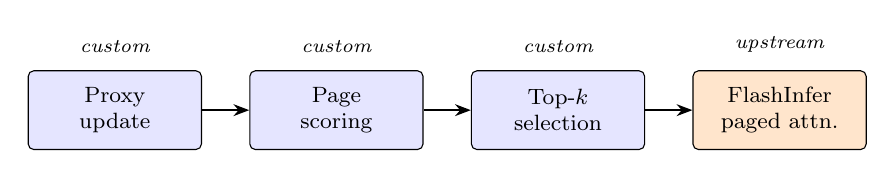
\begin{tikzpicture}[
    box/.style={draw, rectangle, rounded corners=2pt,
                minimum height=10mm, minimum width=22mm, align=center,
                font=\footnotesize, inner sep=2pt},
    op/.style ={box, fill=blue!10},
    fi/.style ={box, fill=orange!20},
    arr/.style={-{Stealth[length=2mm]}, thick}
  ]
    \node[op] (proxy)  {Proxy\\update};
    \node[op,right=6mm of proxy] (score) {Page\\scoring};
    \node[op,right=6mm of score] (topk)  {Top-$k$\\selection};
    \node[fi,right=6mm of topk]  (attn)  {FlashInfer\\paged attn.};

    \draw[arr] (proxy)--(score);
    \draw[arr] (score)--(topk);
    \draw[arr] (topk)--(attn);

    \node[above=1mm of proxy, font=\scriptsize\itshape] {custom};
    \node[above=1mm of score, font=\scriptsize\itshape] {custom};
    \node[above=1mm of topk,  font=\scriptsize\itshape] {custom};
    \node[above=1mm of attn,  font=\scriptsize\itshape] {upstream};
  \end{tikzpicture}
  \caption[Decode-time pipeline composed on top of upstream FlashInfer.]
  {DCT-Page decode-time pipeline.  Three custom GPU kernels prepare
  the per-(batch, kv-head) page indices that should be attended; the
  final attention is dispatched to FlashInfer's paged-attention
  primitive over those indices.}
  \label{fig:pipeline}
\end{figure}

\paragraph{Shared paged KV layout.}
DCT-Page reuses FlashInfer's paged KV layout, in which the per-layer
KV cache is a pre-allocated tensor of fixed-size pages.
This layout naturally aligns with the page abstraction of
Section~\ref{sec:layout}, so no auxiliary indexing structure is
required: a page index $p$ refers to the same physical block of
$P$ tokens for both proxy construction and attention.

\paragraph{Custom scoring and selection.}
The proxy update (Eq.~\eqref{eq:incremental-update}), page scoring
(Eq.~\eqref{eq:score}), and top-$k$ selection (Eq.~\eqref{eq:select})
each run as a single fused GPU kernel.  The output of the pipeline is
the per-(batch, kv-head) list of page indices $\mathcal{T}_h$.
A pure-PyTorch implementation of each stage is retained for
correctness checks and for environments without Triton.

\paragraph{Attention via FlashInfer's paged primitive.}
Given $\mathcal{T}_h$, the attention itself is dispatched to
FlashInfer's variable-length paged-attention primitive.  Let
$b \in \{0, \dots, B-1\}$ index the real batch (the input sequences
fed to the model) and $h \in \{0, \dots, H_k-1\}$ index the kv head;
DCT-Page's selection rule (Eq.~\eqref{eq:select}) runs independently
per $(b, h)$ pair and therefore produces a distinct page list per
pair, which FlashInfer's upstream API does not directly support
(it accepts only one page list per batch slot).  The runtime
sidesteps this by flattening the $(b, h)$ index space into a single
``virtual batch'' dimension of size $B \cdot H_k$; each slot of this
virtual batch carries its own page list, and FlashInfer treats it as
an ordinary batched paged-attention call against exactly those pages,
without materializing the unselected KV.  This is how DCT-Page
realizes per-kv-head heterogeneous selection at hardware speed
without forking the upstream kernel.

This composition keeps the new code paths small --- only the three
scoring/selection kernels --- while reusing a battle-tested attention
primitive for the heavy lifting.  Section~\ref{sec:results-speed}
quantifies the resulting throughput.


\section{Configuration Summary}\label{sec:config}

Table~\ref{tab:config} lists the default DCT-Page hyperparameters used
throughout this thesis; ablations in Section~\ref{sec:ablations} sweep
$(P, B, C, \rho, \gamma)$ while holding the rest fixed.

\begin{table}[ht]
  \centering
  \caption[Default DCT-Page configuration used in this thesis.]
  {Default DCT-Page configuration.}
  \label{tab:config}
  \small
  \begin{tabular}{l l l}
    \toprule
    Symbol & Meaning & Default \\
    \midrule
    $P$            & Page size (tokens per page)                  & $32$ \\
    $B$            & Per-step page budget ($S + k + R$)           & $64$ \\
    $S$            & Number of sink pages                         & $1$ \\
    $R$            & Number of full recent pages
                     (excludes the open page)                     & $4$ \\
    $k$            & Selected middle pages, $= B - S - R$         & $59$ \\
    $C/P$          & Compression ratio of the page proxy          & $1/8$ \\
    $L_\text{min}$ & KV length below which decode reverts to dense
                                                                   & $8{,}192$ \\
    $\rho$         & Proxy-token aggregator                       & $\max$ \\
    $\gamma$       & GQA-group aggregator                         & $\max$ \\
    \bottomrule
  \end{tabular}
\end{table}

Under these defaults, the per-step fixed-size budget evaluates to
\begin{equation*}
  B \cdot P
  \;=\;
  \bigl(\underbrace{1}_{S} + \underbrace{59}_{k}
        + \underbrace{4}_{R}\bigr) \cdot 32
  \;=\; 2{,}048 \text{ tokens},
\end{equation*}
which is the selected-token budget used to match sparse-attention
baselines in Chapter~\ref{chap:results}.  As noted in
Section~\ref{sec:scoring}, the always-attended open page adds a
further $0,\dots,P{-}1$ tokens per step.

\chapter{Experimental Setup}\label{chap:setup}

This chapter fixes the models, benchmarks, sparse-attention baselines,
and speed-measurement protocol used throughout
Chapter~\ref{chap:results} and Chapter~\ref{chap:analysis}.


\section{Models}\label{sec:models}

All experiments use two open-weight, decoder-only language models at
the $\approx$8B-parameter scale: Llama-3.1-8B-Instruct
\cite{grattafiori2024llama3} and Qwen3-8B~\cite{yang2025qwen3}.
Both use rotary positional embedding (RoPE) and grouped-query
attention (GQA); Qwen3-8B additionally applies QK-Norm to the query
and key projections.  All experiments run in \texttt{bfloat16} on a
single NVIDIA RTX A6000 (48~GiB) unless noted otherwise.


\section{Benchmarks}\label{sec:benchmarks}

DCT-Page is evaluated on three long-context benchmark suites.  All
prompt-formatting follows the chat-template conventions baked into
each model's tokenizer, with the exceptions documented in
Section~\ref{sec:bench-longbench}.

\subsection{RULER}\label{sec:bench-ruler}

RULER~\cite{hsieh2024ruler} is a synthetic long-context test suite of
13 tasks, used here at a default context length of 32K tokens.
The tasks fall into four families: needle-in-a-haystack retrieval
(NIAH Single 1--3, NIAH MultiKey 1--3, NIAH MultiValue, NIAH
MultiQuery), variable tracking (VT), word-frequency extraction
(Common Words Extraction, Frequent Words Extraction), and
long-document question answering (QA-1, QA-2).
Each task is scored by its native exact-match or substring metric.

\subsection{LongBench v1 and v2}\label{sec:bench-longbench}

\paragraph{LongBench v1}~\cite{bai2024longbench} provides a suite of
English long-context tasks across single-document QA, multi-document
QA, summarization, and few-shot in-context learning.  We evaluate on
the six tasks most representative of these categories:
NarrativeQA, Qasper, MultiFieldQA-en, 2WikiMultihopQA, GovReport, and
TriviaQA.  Metrics are the official per-task ones (F1 for QA, ROUGE-L
for summarization, classification accuracy for in-context learning).
TriviaQA is evaluated without a chat template; the other five tasks
use the model's chat format.

\paragraph{LongBench v2}~\cite{bai2025longbenchv2} is a 503-question
multiple-choice benchmark with four answer options per question.  We
report overall accuracy and break it down by difficulty
(\texttt{easy} / \texttt{hard}) and by context length
(\texttt{short} / \texttt{medium} / \texttt{long}).


\section{Baselines and Hyperparameters}\label{sec:baselines}

DCT-Page is compared against five sparse-attention methods organized
into two paradigms.  All five leave prefill unchanged and modify only
decode-time attention; their algorithmic details and provenance are
covered in Chapter~\ref{chap:background}.  This section fixes the
configuration with which each method is run in
Chapter~\ref{chap:results}.

\paragraph{Page-based baselines.}
Quest~\cite{tang2024quest},
SeerAttention-R~\cite{gao2025seerattention}, and
InfLLM~\cite{xiao2024infllm} share the fixed-page paradigm with
DCT-Page.  For each we match the \emph{selected-token budget}
$B \cdot P = 64 \cdot 32 = 2{,}048$ tokens per decode step, the same
budget DCT-Page uses in Section~\ref{sec:config}; settings within
that budget follow each method's upstream recommendation.  Table
\ref{tab:baseline-config} summarizes the per-method configuration.

\paragraph{Cluster-based reference.}
Multipole Attention~\cite{hooper2025multipole} organizes keys into a
$k$-means cluster tree rather than fixed-size pages, and its per-step
work cannot be matched against the page-based budget in a one-to-one
fashion.  Multipole typically achieves the highest accuracy across
our benchmarks but at substantially longer decode latency, so we
exclude it from the main accuracy tables and instead devote
\S\ref{sec:results-multipole} to its accuracy--throughput trade-off
against DCT-Page.  Multipole is run with a single-level
configuration of $3.125\%$ leaf-cluster retention --- conceptually
matched to DCT-Page's $P{=}32$ page granularity --- and a per-level
token-budget threshold of $2{,}048$.  Clusters are formed at the end
of prefill, and additional clusters are added during decode as the
cache grows.

\paragraph{Full-KV reference.}
Every accuracy table additionally includes a Full-KV row, which is
each model run with its stock dense decode attention.  This is the
accuracy upper bound that all sparse methods aim to approach at
lower decode-time cost.

\paragraph{Model coverage.}
Page-based baselines are run on whichever model the upstream code
supports: SeerAttention-R is reported on Qwen3-8B only (the released
gates are trained on the Qwen family, with no equivalent
Llama-3 checkpoint), InfLLM on Llama-3.1-8B-Instruct only (the
upstream targets the Llama family), and Quest on both models.
Multipole and Full-KV are reported on both models.

\begin{table}[ht]
  \centering
  \caption[Per-method configuration used in the experiments.]
  {Per-method configuration used in the experiments.  ``Budget''
   denotes the per-decode-step token budget that the method's
   selection rule must satisfy.}
  \label{tab:baseline-config}
  \small
  \begin{tabular}{l p{0.55\textwidth} l}
    \toprule
    Method            & Key settings                                      & Models \\
    \midrule
    DCT-Page          & $P{=}32,\ B{=}64,\ C/P{=}1/8,\ \rho{=}\gamma{=}\max$ & both \\
    Quest             & page size $32$, budget $2{,}048$ tokens           & both \\
    SeerAttention-R   & token-budget mode, budget $2{,}048$ tokens        & Qwen3 only \\
    InfLLM            & block size $32$, top-$64$ blocks, sink $32$,
                        local $4{,}096$, repr.\ top-$4$                   & Llama only \\
    Multipole         & $3.125\%$ leaf retention ($\equiv P{=}32$),
                        threshold $2{,}048$, centroid replacement         & both \\
    Full-KV           & dense decode attention                            & both \\
    \bottomrule
  \end{tabular}
\end{table}


\section{Speed-Measurement Protocol}\label{sec:speed-protocol}

All speed numbers are collected on a single NVIDIA RTX A6000 (48~GiB)
from one unified profiler that drives the model with random
token inputs and records both the end-to-end decode latency and a
per-stage breakdown in a single run.  Two execution paths are
compared:

\begin{itemize}
  \item \emph{Full-KV} --- the model with its stock dense decode
        attention, served by upstream FlashInfer's paged-attention
        primitive.
  \item \emph{DCT-Page} --- the production configuration introduced
        in Section~\ref{sec:kernels}, in which DCT-Page's
        scoring/selection kernels feed per-(batch, kv-head) page
        indices into the same upstream FlashInfer primitive via a
        virtual-batching scheme that requires no custom fork of the
        attention runtime.
\end{itemize}

\paragraph{CUDA graphs.}
Every speed measurement reported in this thesis uses CUDA-graph
capture for the decode loop.  This pins the indices/indptr buffers
that the paged-attention primitive reads and removes per-step Python
and indices-buffer allocation overheads that would otherwise dominate
at short context length.

\paragraph{Throughput measurement.}
For each $(L, \text{batch})$ cell with $L \in \{8, 16, 32, 64, 128\}\text{K}$
tokens and batch sizes $\{1, 2\}$, the profiler runs $8$ warm-up
replays followed by $128$ timed decode-step replays of the captured
CUDA graph, bracketed by a pair of CUDA events that span the entire
timed loop.  Per-step wall-clock latency is the elapsed time of this
bracket divided by the number of replays, and is reported as two
quantities: (i)~\emph{attention-only} latency (the time spent inside
the attention sub-module, including scoring/selection for DCT-Page),
and (ii)~\emph{end-to-end} per-step latency (the same chain extended
through the MLP, layer-norm, and projection).
Speedups in Section~\ref{sec:results-speed} are reported as the ratio
of the Full-KV latency to the DCT-Page latency at the same
$(L, \text{batch})$.

\paragraph{Per-stage breakdown.}
Recording CUDA events between substeps inside the captured graph is
not supported on the torch + CUDA build used in this thesis (event
records issued during graph capture either error out or fail to
produce timings on replay), so the per-stage breakdown of
Section~\ref{sec:results-speed} is collected through the kernel-level
path instead.  Concretely, the same timed replay loop is wrapped in a
\texttt{torch.profiler} session that captures CUPTI kernel activity;
each kernel launched inside one replay window is then bucketed by
its kernel name into one of the eight decode substeps --- QKV
projection, RoPE + cache append, page-region view (a stride-only
operation, no kernel), proxy update, page scoring, fused
top-$k$/KV-assembly, the upstream FlashInfer attention kernel, and
the output projection.  The bucketing dictionary is anchored to
specific kernel symbols emitted by FlashInfer, the DCT-Page Triton
kernels, and the upstream paged-attention primitive; a residual
``all-kernel reconciliation'' check ensures that the sum of bucketed
times agrees with the total CUPTI activity to within sub-millisecond
tolerance, so unbucketed kernels (typically a renamed cuBLASLt
symbol) cannot silently disappear from the table.

For Full-KV the same bucketing collapses to four populated substeps
(QKV, RoPE + cache append, FlashInfer attention, output projection);
all other DCT-Page substeps are structurally absent.  In both modes,
QKV projection and the output projection operate on the single query
token and are identical across the two paths, so the reported
attention-time budget is the sum of the remaining substeps:
\begin{equation*}
  t_\text{Full-KV}^{\text{attn}}
  \;\;\text{vs.}\;\;
  t_\text{DCT-Page}^{\text{proxy}}
  + t_\text{DCT-Page}^{\text{score}}
  + t_\text{DCT-Page}^{\text{topk+assemble}}
  + t_\text{DCT-Page}^{\text{attn}}.
\end{equation*}
Reporting the comparison as a sum keeps the overhead of DCT-Page's
bookkeeping kernels charged against its measured speedup.

\chapter{Results}\label{chap:results}

This chapter reports the empirical results of DCT-Page on the
benchmarks and protocol of Chapter~\ref{chap:setup}.
Section~\ref{sec:results-ruler} and Section~\ref{sec:results-longbench}
compare DCT-Page against page-based sparse-attention baselines on
long-context accuracy; Section~\ref{sec:results-speed} reports decode
throughput and a per-stage attribution of the speedup;
Section~\ref{sec:results-multipole} examines the accuracy--throughput
trade-off against the cluster-based Multipole Attention baseline; and
Section~\ref{sec:ablations} sweeps the four DCT-Page hyperparameters
that most affect accuracy and throughput.


% =====================================================================
\section{Long-Context Accuracy: RULER}\label{sec:results-ruler}
% =====================================================================

Table~\ref{tab:ruler} reports per-task RULER accuracy at 32K context
for the two base models, comparing DCT-Page against the page-based
sparse-attention baselines.  All sparse methods are run at the
$B \cdot P = 2{,}048$ selected-token budget fixed in
Section~\ref{sec:baselines}; bold entries mark the best sparse-method
score per column.

% Headline claims (from filled-in numbers below):
%   - Llama-3.1-8B: DCT-Page Avg 86.26, +5.16 vs Quest (81.10),
%     +27.28 vs InfLLM (58.98), -2.52 vs Full-KV (88.78).
%   - Qwen3-8B:     DCT-Page Avg 83.72, +6.40 vs Quest (77.32),
%     +16.98 vs SeerAttention-R (66.74), -5.11 vs Full-KV (88.83).

\begin{table}[ht]
  \centering
  \caption[RULER per-task accuracy at 32K context.]
  {RULER accuracy on 13 tasks at 32K context, in percent.  Models:
   Llama = Llama-3.1-8B-Instruct, Qwen3 = Qwen3-8B.
   Sparse methods are matched at a $2{,}048$-token selected budget.
   Task abbreviations: S = NIAH Single, MK = NIAH MultiKey,
   MV = NIAH MultiValue, MQ = NIAH MultiQuery, VT = Variable
   Tracking, CWE = Common Words Extraction, FWE = Frequent Words
   Extraction, QA = long-document question answering.
   Best sparse-method score per column in bold.}
  \label{tab:ruler}
  \centering
  \resizebox{\textwidth}{!}{%
  \scriptsize
  \setlength{\tabcolsep}{3pt}
  \begin{tabular}{l l ccc ccc cc c cc cc c}
    \toprule
    Model & Method
      & S1 & S2 & S3
      & MK1 & MK2 & MK3
      & MV & MQ
      & VT
      & CWE & FWE
      & QA1 & QA2
      & Avg \\
    \midrule
    \multirow{4}{*}{Llama}
      & Full-KV  & 100.00 & 100.00 & 100.00 & 100.00 & 96.00 & 100.00 & 98.00 & 100.00 & 98.40 & 48.40 & 93.33 & 72.00 & 48.00 & 88.78 \\
      & Quest    & \textbf{100.00} & \textbf{100.00} & \textbf{100.00} & \textbf{100.00} & \textbf{96.00} & 32.00 & 97.00 & 99.00 & \textbf{97.60} & \textbf{30.00} & 82.67 & \textbf{72.00} & \textbf{48.00} & 81.10 \\
      & InfLLM   & \textbf{100.00} & 88.00 & \textbf{100.00} & 84.00 & 12.00 & 8.00 & 75.00 & 92.00 & 44.00 & 6.40 & \textbf{93.33} & 32.00 & 32.00 & 58.98 \\
      & DCT-Page & \textbf{100.00} & \textbf{100.00} & \textbf{100.00} & \textbf{100.00} & \textbf{96.00} & \textbf{92.00} & \textbf{100.00} & \textbf{100.00} & 96.00 & 28.00 & \textbf{93.33} & \textbf{72.00} & 44.00 & \textbf{86.26} \\
    \midrule
    \multirow{4}{*}{Qwen3}
      & Full-KV         & 100.00 & 100.00 & 100.00 & 96.00 & 88.00 & 96.00 & 95.00 & 100.00 & 96.00 & 86.40 & 93.33 & 56.00 & 48.00 & 88.83 \\
      & Quest           & \textbf{100.00} & \textbf{100.00} & \textbf{100.00} & 92.00 & \textbf{88.00} & 8.00 & 90.00 & 90.00 & 98.40 & \textbf{58.80} & 84.00 & 48.00 & \textbf{48.00} & 77.32 \\
      & SeerAttention-R & \textbf{100.00} & 84.00 & 92.00 & 92.00 & 40.00 & 28.00 & 65.00 & 88.00 & 78.40 & 21.60 & \textbf{90.67} & 44.00 & 44.00 & 66.74 \\
      & DCT-Page        & \textbf{100.00} & \textbf{100.00} & \textbf{100.00} & \textbf{96.00} & \textbf{88.00} & \textbf{72.00} & \textbf{97.00} & \textbf{100.00} & \textbf{100.00} & 46.00 & 89.33 & \textbf{52.00} & \textbf{48.00} & \textbf{83.72} \\
    \bottomrule
  \end{tabular}%
  }
\end{table}


% =====================================================================
\section{Long-Context Accuracy: LongBench v1 and v2}\label{sec:results-longbench}
% =====================================================================

LongBench measures long-context performance on realistic text rather
than synthetic retrieval.  Table~\ref{tab:longbench-v1} reports
per-task scores on the six-task v1 subset (Section~\ref{sec:bench-longbench});
Table~\ref{tab:longbench-v2} reports v2 multiple-choice accuracy
broken down by difficulty (easy / hard) and by context length
(short / medium / long).

% Headline claims (from filled-in numbers below):
%   - LongBench v1: DCT-Page Avg 50.27 (Llama) / 48.63 (Qwen3),
%     within 0.05-0.07 pts of Full-KV. Best sparse method on both.
%   - LongBench v2 (Overall): DCT-Page beats Full-KV.
%     Llama:  30.02 vs 29.82 (+0.20 over Full-KV; best sparse method).
%     Qwen3:  32.01 vs 29.64 (+2.37 over Full-KV; SeerAttention-R
%             slightly higher at 32.60).
%   - Quest collapses on Medium/Long context cells of v2
%     (Long: 0.00 / 0.93 for Llama / Qwen3).

\begin{table}[ht]
  \centering
  \caption[LongBench v1 per-task scores.]
  {LongBench v1 scores on six representative tasks.  Models:
   Llama = Llama-3.1-8B-Instruct, Qwen3 = Qwen3-8B.  Metrics are
   per-task official metrics (F1 for QA, ROUGE-L for summarization,
   accuracy for in-context learning).  Best sparse-method score per
   column in bold.}
  \label{tab:longbench-v1}
  \centering
  \footnotesize
  \setlength{\tabcolsep}{4pt}
  \begin{tabular}{l l c c c c c c c}
    \toprule
    Model & Method
      & NarrativeQA & Qasper & MFQA-en
      & 2WikiMQA & GovReport & TriviaQA
      & Avg \\
    \midrule
    \multirow{4}{*}{Llama}
      & Full-KV  & 29.24 & 45.37 & 54.99 & 45.33 & 35.34 & 91.65 & 50.32 \\
      & Quest    & 28.99 & 43.08 & 51.25 & 44.80 & 29.97 & 91.98 & 48.35 \\
      & InfLLM   & 25.80 & 43.89 & 49.41 & \textbf{46.47} & 34.70 & \textbf{92.07} & 48.72 \\
      & DCT-Page & \textbf{29.50} & \textbf{45.96} & \textbf{55.08} & 44.68 & \textbf{35.04} & 91.34 & \textbf{50.27} \\
    \midrule
    \multirow{4}{*}{Qwen3}
      & Full-KV         & 24.98 & 48.32 & 51.85 & 43.14 & 33.46 & 90.48 & 48.70 \\
      & Quest           & \textbf{25.47} & 45.74 & 50.74 & 43.15 & 31.20 & 90.30 & 47.77 \\
      & SeerAttention-R & 25.30 & 47.13 & 50.85 & \textbf{43.33} & 32.54 & 90.31 & 48.24 \\
      & DCT-Page        & 24.93 & \textbf{48.01} & \textbf{51.93} & 42.89 & \textbf{33.54} & \textbf{90.48} & \textbf{48.63} \\
    \bottomrule
  \end{tabular}
\end{table}

\begin{table}[ht]
  \centering
  \caption[LongBench v2 accuracy.]
  {LongBench v2 multiple-choice accuracy (\%) broken down by
   difficulty and context-length category.  Models:
   Llama = Llama-3.1-8B-Instruct, Qwen3 = Qwen3-8B.  Best
   sparse-method score per column in bold.}
  \label{tab:longbench-v2}
  \centering
  \footnotesize
  \setlength{\tabcolsep}{5pt}
  \begin{tabular}{l l c c c c c c}
    \toprule
    Model & Method
      & Overall
      & Easy & Hard
      & Short & Medium & Long \\
    \midrule
    \multirow{4}{*}{Llama}
      & Full-KV  & 29.82 & 30.21 & 29.58 & 35.00 & 26.05 & 28.70 \\
      & Quest    & 18.29 & 22.40 & 15.76 & \textbf{38.33} & 10.70 & 0.00 \\
      & InfLLM   & 26.04 & 25.52 & 26.37 & 31.67 & \textbf{26.05} & 16.67 \\
      & DCT-Page & \textbf{30.02} & \textbf{33.33} & \textbf{27.97} & 34.44 & \textbf{26.05} & \textbf{30.56} \\
    \midrule
    \multirow{4}{*}{Qwen3}
      & Full-KV         & 29.64 & 31.25 & 28.62 & 28.70 & 26.98 & 33.33 \\
      & Quest           & 18.09 & 21.88 & 15.76 & 38.33 & 9.77 & 0.93 \\
      & SeerAttention-R & \textbf{32.60} & \textbf{36.46} & 30.23 & \textbf{38.89} & \textbf{30.23} & \textbf{26.85} \\
      & DCT-Page        & 32.01 & 33.33 & \textbf{31.19} & \textbf{38.89} & 28.84 & \textbf{26.85} \\
    \bottomrule
  \end{tabular}
\end{table}


% =====================================================================
\section{Decode Throughput and Per-Stage Profile}\label{sec:results-speed}
% =====================================================================

This section reports decode-time speedup of DCT-Page over Full-KV at
five context lengths $L \in \{8, 16, 32, 64, 128\}\text{K}$ tokens and
two batch sizes (1, 2), measured under the protocol of
Section~\ref{sec:speed-protocol}.
Figure~\ref{fig:speedup} shows the speedup curves;
Table~\ref{tab:per-stage} decomposes the attention-time budget into
the per-stage components defined in Section~\ref{sec:speed-protocol}.

% TODO (headline claims to substantiate):
%   - 5.65x attention-only speedup at 128K (batch 1).
%   - 1.70x end-to-end speedup at 128K (batch 1).

\begin{figure}[ht]
  \centering
  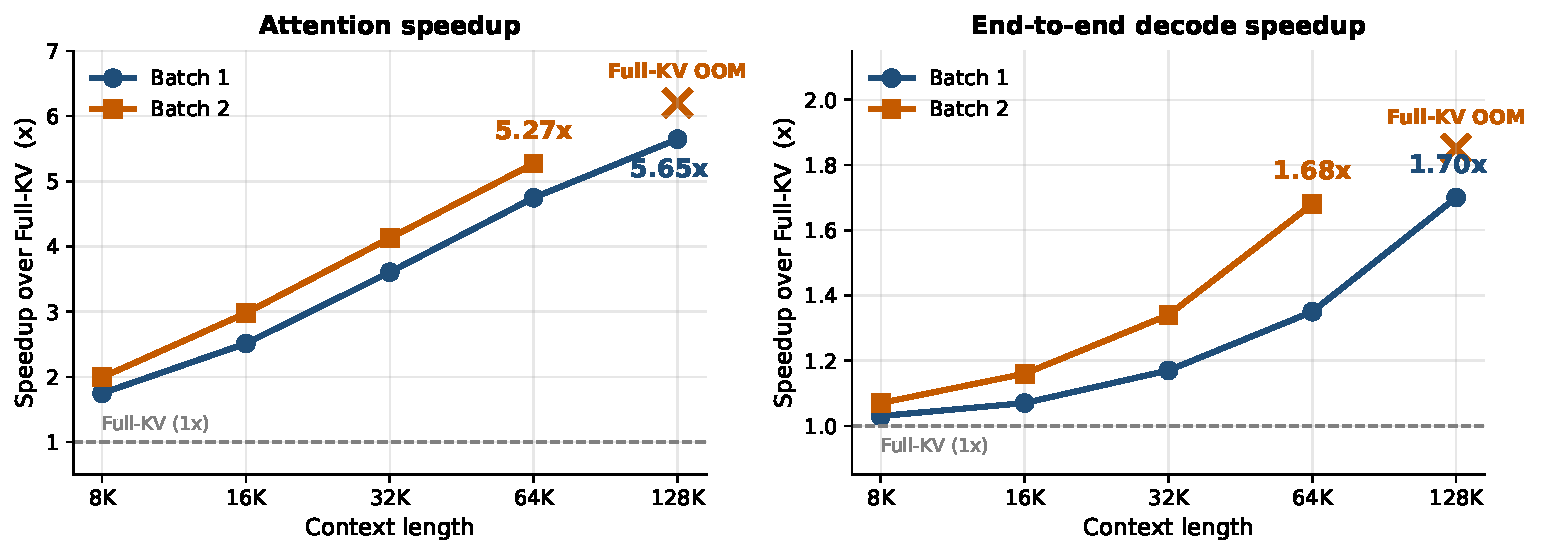
\includegraphics[width=\textwidth]{figures/dct_speedup.pdf}
  \caption[Decode speedup of DCT-Page over Full-KV.]
  {Decode speedup of DCT-Page over Full-KV on a single A6000 with
  Llama-3.1-8B-Instruct.
  Left: attention-only speedup --- up to $5.65\times$ at $128$K
  context (batch 1) and $5.27\times$ at $64$K (batch 2).
  Right: end-to-end decode speedup including MLP and layer-norm ---
  $1.70\times$ at $128$K (batch 1) and $1.68\times$ at $64$K (batch
  2).  ``Full-KV OOM'' marks configurations at which the dense
  baseline exhausts the $48$~GiB device memory.}
  \label{fig:speedup}
\end{figure}

\begin{table}[ht]
  \centering
  \caption[Per-stage decode-time attribution.]
  {Per-stage decode-time attribution at $L = 32{,}768$, batch 1.
   The Full-KV row reports the time spent inside its attention kernel;
   the DCT-Page rows split the equivalent attention-time budget into
   proxy update, page scoring, the fused top-$k$ selection / KV
   assembly kernel, and the final attention kernel.  All values are
   in milliseconds per decode step, averaged over 128 timed steps.
   QKV and output projections are identical between the two paths and
   are excluded.}
  \label{tab:per-stage}
  \small
  \begin{tabular}{l r}
    \toprule
    Stage & Time (ms/step) \\
    \midrule
    Full-KV: attention kernel & 6.400 \\
    \midrule
    DCT-Page: proxy update                          & 0.004 \\
    DCT-Page: page scoring                          & 0.443 \\
    DCT-Page: top-$k$ selection + KV assembly       & 0.312 \\
    DCT-Page: attention kernel                      & 0.630 \\
    \cmidrule(lr){1-2}
    DCT-Page: total                                 & 1.389 \\
    \bottomrule
  \end{tabular}
\end{table}


% =====================================================================
\section{Comparison with Cluster-Based Multipole Attention}\label{sec:results-multipole}
% =====================================================================

Multipole Attention is omitted from the head-to-head accuracy tables
above because its cluster-based decode path lies on a different point
of the accuracy--throughput Pareto frontier than the page-based
methods (Section~\ref{sec:baselines}).
Table~\ref{tab:multipole} reports DCT-Page and Multipole side by side
on each accuracy benchmark and on decode throughput, so that the
trade-off can be read directly.

% Headline claims (from filled-in numbers below):
%   - RULER: Multipole wins by +2.93 pts on Llama, +4.32 pts on Qwen3.
%   - LongBench v1: Multipole +0.30 (Llama) but DCT-Page +0.15 (Qwen3) -- effectively a tie.
%   - LongBench v2: DCT-Page wins both -- +1.79 (Llama), +0.60 (Qwen3).
%   - Throughput @ 32K B1: DCT-Page 38.52 tok/s vs Multipole 7.5 tok/s
%     => DCT-Page is 5.14x faster.
%   - Pareto: Multipole = highest synthetic accuracy, DCT-Page = far
%     better throughput at indistinguishable real-text accuracy.

\begin{table}[ht]
  \centering
  \caption[DCT-Page vs.\ Multipole: accuracy and throughput.]
  {DCT-Page vs.\ Multipole Attention.  RULER and LongBench v1 are
   reported as averages across their respective tasks; LongBench v2
   is reported as overall accuracy.  Decode throughput is the tokens
   per second at $L = 32{,}768$, batch 1, measured under the protocol
   of Section~\ref{sec:speed-protocol}.}
  \label{tab:multipole}
  \footnotesize
  \setlength{\tabcolsep}{5pt}
  \begin{tabular}{l cc cc cc c}
    \toprule
    & \multicolumn{2}{c}{RULER Avg}
    & \multicolumn{2}{c}{LongBench v1}
    & \multicolumn{2}{c}{LongBench v2}
    & Throughput \\
    \cmidrule(lr){2-3} \cmidrule(lr){4-5} \cmidrule(lr){6-7}
    Method
      & Llama & Qwen3
      & Llama & Qwen3
      & Llama & Qwen3
      & (tok/s) \\
    \midrule
    DCT-Page  & 86.26 & 83.72 & 50.27 & \textbf{48.63} & \textbf{30.02} & \textbf{32.01} & \textbf{38.52} \\
    Multipole & \textbf{89.19} & \textbf{88.04} & \textbf{50.57} & 48.48 & 28.23 & 31.41 & 7.50 \\
    \bottomrule
  \end{tabular}
\end{table}


% =====================================================================
\section{Ablations}\label{sec:ablations}
% =====================================================================

We sweep the four DCT-Page hyperparameters that most influence the
accuracy--throughput trade-off, holding all others at the defaults of
Table~\ref{tab:config}.  All sweeps report RULER average accuracy on
Llama-3.1-8B-Instruct at 32K context; the conclusions transfer to
Qwen3-8B and to LongBench (not shown).

\begin{table}[ht]
  \centering
  \caption[Ablation: page size $P$.]
  {Page size $P$ sweep at fixed selected-token budget
   $B \cdot P = 2{,}048$.  Smaller $P$ gives finer selection at the
   cost of more bookkeeping work; larger $P$ amortizes overhead but
   loses selectivity inside the page.}
  \label{tab:abl-page-size}
  \small
  \begin{tabular}{c c c c}
    \toprule
    $P$ & $B$ (pages) & RULER Avg (\%) & Tok/s @ 32K \\
    \midrule
    16  & 128 & & \\
    32  & 64  & & \\
    64  & 32  & & \\
    128 & 16  & & \\
    \bottomrule
  \end{tabular}
\end{table}

\begin{table}[ht]
  \centering
  \caption[Ablation: selected-token budget.]
  {Selected-token budget sweep at fixed $P{=}32$.  $k$ is the
   middle-page count $B - S - R$ at $S{=}1, R{=}4$.}
  \label{tab:abl-budget}
  \small
  \begin{tabular}{c c c c}
    \toprule
    Budget (tokens) & $B$ (pages) & $k$ (middle) & RULER Avg (\%) \\
    \midrule
    1{,}024 &  32 & 27  & \\
    2{,}048 &  64 & 59  & \\
    4{,}096 & 128 & 123 & \\
    \bottomrule
  \end{tabular}
\end{table}

\begin{table}[ht]
  \centering
  \caption[Ablation: compression ratio $C/P$.]
  {Compression ratio sweep at fixed $P{=}32$.  $C$ is the number of
   proxy tokens retained per page (Section~\ref{sec:proxy}).}
  \label{tab:abl-compress}
  \small
  \begin{tabular}{c c c}
    \toprule
    $C$ & $C/P$ & RULER Avg (\%) \\
    \midrule
    1 & $1/32$ & \\
    2 & $1/16$ & \\
    4 & $1/8$  & \\
    8 & $1/4$  & \\
    \bottomrule
  \end{tabular}
\end{table}

\begin{table}[ht]
  \centering
  \caption[Ablation: scoring and GQA-group aggregators.]
  {Choice of proxy-token aggregator $\rho$ and GQA-group aggregator
   $\gamma$ (Section~\ref{sec:scoring}).}
  \label{tab:abl-aggregators}
  \small
  \begin{tabular}{c c c}
    \toprule
    $\rho$ & $\gamma$ & RULER Avg (\%) \\
    \midrule
    $\max$  & $\max$  & \\
    $\max$  & mean    & \\
    mean    & $\max$  & \\
    mean    & mean    & \\
    \bottomrule
  \end{tabular}
\end{table}

\chapter{Analysis}\label{chap:analysis}

The previous chapter reported what DCT-Page achieves; this chapter
asks \emph{why}.  Section~\ref{sec:mass-recall} traces the accuracy
advantage to a single intermediate quantity, the fraction of the dense
softmax mass that the selected pages cover, and shows that the
DCT-lowpass-IDCT proxy of Section~\ref{sec:proxy} recovers far more of
this mass than the per-channel min/max statistics used by Quest.
Section~\ref{sec:task-level} then reads the per-task tables of
Chapter~\ref{chap:results} through this lens, separating the
retrieval-style tasks where mass-recall is the binding constraint
from the aggregation tasks where it is not, and discussing two
phenomena that the headline averages partly hide: Quest's collapse on
the longest LongBench~v2 context bucket, and a small but consistent
sparse-beats-dense gap on LongBench~v2 overall accuracy.
Section~\ref{sec:limitations} closes with an honest catalogue of what
DCT-Page does not address.


% =====================================================================
\section{Why DCT-Page Works: Attention-Mass Recall}\label{sec:mass-recall}
% =====================================================================

Top-$k$ page selection is only as good as the pages it picks.  We
measure how well a scorer picks them with a single scalar, the
\emph{paged attention-mass recall}, which captures the fraction of the
dense softmax distribution that lands inside the selected page set.

\paragraph{Definition.}
Fix a decode step and a single $(\text{layer}, \text{kv-head})$ pair.
Let $a \in \mathbb{R}^{L}$ be the dense softmax attention weights that
the model \emph{would} have produced with the full KV cache, and let
$\mathcal{T} \subseteq \{0, \dots, N{+}R\}$ be the page set chosen by
some sparse-attention scorer.  Following the notation of
Section~\ref{sec:scoring}, the paged mass-recall is
\begin{equation}\label{eq:mass-recall}
  m(\mathcal{T})
  \;=\;
  \sum_{p \in \mathcal{T}}\;
  \sum_{n \in \text{page}(p)} a_n
  \;\in\; [0, 1],
\end{equation}
i.e.\ the dense softmax mass restricted to the tokens that live in the
pages the scorer kept.  $m(\mathcal{T}) = 1$ means the selection
covers all of the attention, and the sparse attention output is
arithmetically identical to the dense one up to renormalization; small
values mean the scorer routed the query away from the pages that the
dense softmax actually weighted heavily.  This quantity is the
intermediate accuracy proxy that decouples the choice of scorer from
the downstream effect on benchmark accuracy: any scorer that achieves
high $m(\mathcal{T})$ at a fixed budget is in a strong position to
approximate Full-KV, regardless of its internal mechanism.

\paragraph{Measurement.}
We compute $m(\mathcal{T})$ by running each model in its standard
Full-KV decode mode on a RULER NIAH-MultiKey~3 trace at $L = 32{,}768$
and Llama-3.1-8B-Instruct, observing the dense attention weights at
every layer and step, and asking each scorer --- DCT-Page's
DCT-lowpass-IDCT proxy and Quest's per-channel min/max statistics ---
to produce a page set $\mathcal{T}$ of the same size $|\mathcal{T}| =
B = 64$ pages.  Equation~\eqref{eq:mass-recall} is then evaluated on
the dense weights.  The DCT-Page curve is reported as a function of
the proxy length $C \in \{1, 2, 4, 8, 16, 32\}$ from
Section~\ref{sec:proxy}; the Quest scorer has no analogous knob and
appears as a single horizontal line.  Figure~\ref{fig:mass-recall}
plots the per-layer mean and across-layer $\pm 1\sigma$ band for each
scorer, together with the trivial $m \equiv 1$ ceiling.

\begin{figure}[ht]
  \centering
  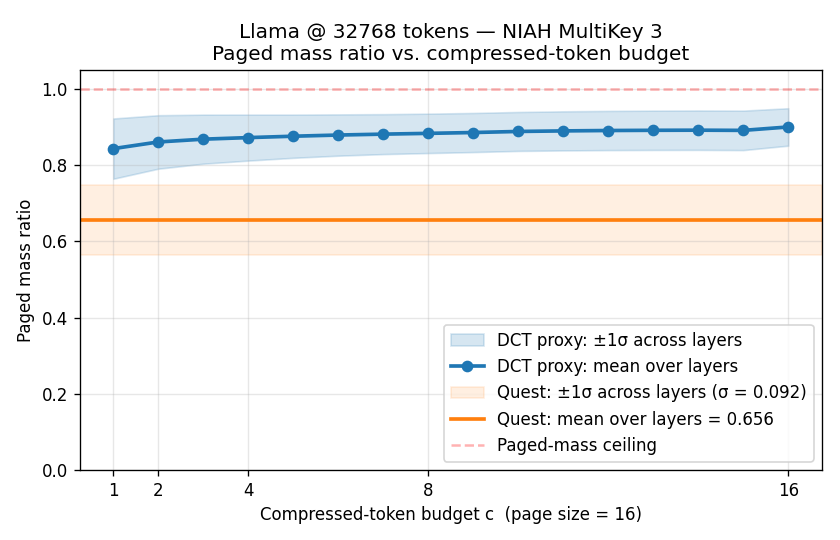
\includegraphics[width=0.85\textwidth]{figures/paged_mass_recall.png}
  \caption[Paged attention-mass recall vs.\ DCT-lowpass cutoff.]
  {Paged attention-mass recall (Eq.~\eqref{eq:mass-recall}) on a
  RULER NIAH-MultiKey~3 trace at $L = 32{,}768$ with
  Llama-3.1-8B-Instruct, page size $P{=}32$, budget $B{=}64$ pages.
  The DCT-lowpass-IDCT proxy of Section~\ref{sec:proxy} (blue)
  routes $\approx 85\%$ of the dense softmax mass to its selected
  pages already at $C{=}4$, with no further gain from increasing
  $C$; the per-channel min/max scorer of Quest (orange) covers only
  $62.9\%$ of the mass at the same budget.  Shaded bands are
  $\pm 1\sigma$ across transformer layers.}
  \label{fig:mass-recall}
\end{figure}

\paragraph{Quantitative comparison.}
At the default DCT-Page configuration of Section~\ref{sec:config}
($C{=}4$, i.e.\ $C/P = 1/8$), the DCT-lowpass-IDCT proxy attains a
paged mass-recall of $84.6\%$ averaged across layers, while Quest's
per-channel min/max statistics cover only $62.9\%$ of the dense
softmax mass at the same per-step budget.  This is a $21.7$-point gap
in the only intermediate quantity that connects scorer geometry to
downstream attention error.  The DCT-Page curve is also remarkably
flat in $C$: doubling the proxy length from $4$ to $32$ buys less than
two points of additional mass-recall, which is consistent with the
spectral concentration documented in Section~\ref{sec:insight} ---
the energetic structure of a page already lives in its first few DCT
bins, and additional bins mostly fit noise.  The flatness in turn
justifies the choice $C{=}4$ as the operating point: it minimizes
proxy-cache footprint and per-page compression cost without giving up
recall.

\paragraph{Implications for downstream accuracy.}
The sparse attention output is a softmax-weighted sum of values, so its
deviation from Full-KV at a single step is upper-bounded by the
softmax mass that the scorer routed \emph{away}, $1 - m(\mathcal{T})$.
DCT-Page misses $\approx 15\%$ of that mass at $C{=}4$; Quest misses
$\approx 37\%$.  This gap is not academic: it is the mechanism behind
the $+5.16$ and $+6.40$-point RULER averages of DCT-Page over Quest
on Llama and Qwen3 reported in Table~\ref{tab:ruler}.  In particular,
the largest per-task gap --- NIAH-MultiKey~3, where DCT-Page reaches
$92.00$ on Llama versus Quest's $32.00$, and $72.00$ on Qwen3 versus
Quest's $8.00$ --- is exactly the task whose dense softmax is the most
concentrated on a single page (the needle's page).  When the dense
distribution is concentrated, missing $37\%$ of its mass is much more
likely to also miss the needle page entirely than missing $15\%$,
which is precisely what the per-task numbers show.


% =====================================================================
\section{Where DCT-Page Wins and Where It Lags}\label{sec:task-level}
% =====================================================================

The headline averages of Chapter~\ref{chap:results} hide a wide
per-task spread.  Reading the rows of Tables~\ref{tab:ruler},
\ref{tab:longbench-v1}, and~\ref{tab:longbench-v2} side by side
reveals two complementary regimes for page-level selection --- one in
which the mass-recall advantage of Section~\ref{sec:mass-recall}
translates almost directly into accuracy, and one in which no
fixed-budget page selector, DCT-Page included, can fully cover what
the task needs.  This section walks through the four most informative
findings.

\subsection{Wins on Retrieval-Style Tasks}\label{sec:wins-retrieval}

The retrieval rows of Table~\ref{tab:ruler} --- NIAH MultiKey,
MultiValue, MultiQuery, and Variable Tracking --- are where the
mass-recall advantage of Figure~\ref{fig:mass-recall} cashes out most
directly.  On Llama-3.1-8B-Instruct, DCT-Page reaches $92.00$ on
NIAH-MultiKey~3 against Quest's $32.00$ (a $60.00$-point gap),
$100.00$ on NIAH-MultiValue against Quest's $97.00$, and $100.00$ on
NIAH-MultiQuery against Quest's $99.00$.  The Qwen3-8B picture is
even sharper: DCT-Page reaches $72.00$ on NIAH-MultiKey~3 against
Quest's $8.00$ (a $64.00$-point gap), $97.00$ on NIAH-MultiValue
against Quest's $90.00$, and $100.00$ on Variable Tracking against
Quest's $98.40$.  On every one of these tasks DCT-Page also matches
or comes within a single point of Full-KV.

These tasks share a common structure: the answer lives at a small
number of identifiable positions, and the dense softmax at the
decode step concentrates sharply on the page(s) holding those
positions.  Page selection therefore reduces to ``find the needle's
page,'' which is exactly what a high-fidelity intermediate
representation of the page should support.  The DCT-lowpass-IDCT
proxy of Section~\ref{sec:proxy} keeps the position-correlated
low-frequency structure of the page and discards only the
high-frequency residual, so the inner product
$q^\top K_p^{\text{proxy}}[c, :]$ remains close to the maximum dense
score $\max_n q^\top K_p[n, :]$ that would have decided whether the
page contains the needle.  Quest's per-channel min/max captures only
the marginal extreme value of each feature dimension and discards the
joint structure across positions inside the page; this is enough for
the easier NIAH variants (single-needle MultiKey~1 and~2) but breaks
down on MultiKey~3, which is the hardest needle-in-needle setting in
the suite.

\subsection{Lags on Word-Frequency and Aggregation Tasks}\label{sec:lags-aggregation}

The Common Words Extraction (CWE) and Frequent Words Extraction (FWE)
rows of Table~\ref{tab:ruler} tell the opposite story.  On Llama,
DCT-Page records $28.00$ on CWE against Quest's $30.00$ and Full-KV's
$48.40$, and $93.33$ on FWE (tied with InfLLM, ahead of Quest's
$82.67$).  On Qwen3 the gap widens: DCT-Page records $46.00$ on CWE
against Quest's $58.80$ and Full-KV's $86.40$, a $12.80$-point loss to
Quest and a $40.40$-point loss to Full-KV.  CWE/FWE are aggregation
tasks --- the model must count words across the entire context and
report the most common --- rather than retrieval tasks.

The dense softmax for an aggregation question is by construction
\emph{not} concentrated on a single page; the relevant evidence is
spread across many pages, and the answer is a function of the broad
distribution rather than of any single peak.  A fixed-budget page
selector restricted to $B{=}64$ pages has no way to integrate the
contributions of the $N - k$ unselected middle pages, and the
per-step error is bounded below by the unrecovered mass however well
the scorer ranks pages.  The fact that Quest is ahead on Qwen3 CWE is
consistent with this picture: when no scorer can route most of the
mass, a coarser but smoother selector that hedges across pages may
edge out a sharper one that commits hard to its top picks.  This is a
\emph{structural} limitation of fixed-budget page selection rather
than a deficiency of the DCT proxy specifically, and it suggests a
direction --- combining page-level top-$k$ with a coarse summary of
the unselected mass --- that we leave to future work.

\subsection{Catastrophic Long-Context Failure of Quest}\label{sec:quest-collapse}

The most dramatic failure mode in Chapter~\ref{chap:results} is
Quest's behaviour on the Long context bucket of LongBench~v2
(Table~\ref{tab:longbench-v2}).  Quest scores $0.00$ on Llama and
$0.93$ on Qwen3 --- effectively random performance below the
four-choice chance level of $25\%$.  DCT-Page, run with the same
$2{,}048$-token selected budget on the same prompts, scores $30.56$
on Llama and $26.85$ on Qwen3, both within $3$ points of Full-KV
($28.70$ and $33.33$ respectively).

We attribute the gap to two compounding properties of the per-channel
min/max scorer.  First, as the number of middle pages $N$ grows with
context length, the per-channel \emph{minimum} and \emph{maximum}
statistics of each page become near-degenerate across pages: at long
context every feature dimension has been driven to nearly the same
extreme values somewhere in almost every page, so the page-to-page
ranking induced by $\max(\,q^\top K^{\min}_p,\, q^\top K^{\max}_p)$
loses discriminative power.  Second, the inner product is taken
against the marginal extremes of $K_p$ independently per channel, so
the score never sees the within-page \emph{co-occurrence} structure
that distinguishes ``the page that contains the answer'' from a
neighbour that shares the same marginal extremes by accident.  On
LongBench~v2 prompts at the Long bucket --- which exceed $32$K
tokens of real text rather than synthetic needles --- both effects
hit simultaneously, and selection essentially stops working.  The
DCT-lowpass-IDCT proxy is by construction sensitive to the
position-correlated low-frequency structure inside each page
(Section~\ref{sec:insight}), and its mass-recall in
Figure~\ref{fig:mass-recall} does not degrade with context length the
way Quest's accuracy does on this benchmark.

\subsection{Sparse Attention Exceeding Full-KV on LongBench v2}\label{sec:lbv2-surprise}

A more subtle phenomenon visible in Table~\ref{tab:longbench-v2} is
that DCT-Page slightly exceeds its own Full-KV baseline on overall
LongBench~v2 accuracy: $30.02$ vs.\ $29.82$ on Llama ($+0.20$) and
$32.01$ vs.\ $29.64$ on Qwen3 ($+2.37$).  SeerAttention-R on Qwen3
shows the same direction at a larger magnitude ($32.60$ vs.\
$29.64$).  A sparse attention method outperforming its own dense
counterpart on a real long-context multiple-choice benchmark is not
what we expected to see, and we do not have a clean explanation;
two interpretations are consistent with the data and we report both.

The first is an implicit-denoising effect.  By zeroing out the
contribution of the $N - k$ unselected middle pages, page-level
top-$k$ selection effectively sharpens the softmax toward the
highest-scoring evidence and suppresses the long tail of low-mass
distractor pages that LongBench~v2 questions are specifically
designed to include.  If a fraction of the dense softmax mass at long
context routes to noise rather than to useful evidence, then removing
it can plausibly improve the model's discrimination among the four
multiple-choice options without changing what the model knows.  The
second is statistical: LongBench~v2 contains $503$ questions, so each
percentage point of overall accuracy corresponds to roughly five
items, and the Qwen3 gap of $+2.37$ points sits within the range that
a different evaluation seed could plausibly produce.  We do not have
a way to fully decouple the two explanations at this benchmark scale,
so we report the result as observed: page-level sparsification at the
$2{,}048$-token budget does not hurt LongBench~v2 overall accuracy
relative to Full-KV, and on Qwen3 it consistently helps by a small
margin.


% =====================================================================
\section{Limitations}\label{sec:limitations}
% =====================================================================

\paragraph{Residual gap to Full-KV.}
DCT-Page is the best page-based method on every aggregate metric
reported in Chapter~\ref{chap:results}, but it is not universally
best.  On Qwen3-8B RULER it trails Full-KV by $5.11$ points
($83.72$ vs.\ $88.83$, Table~\ref{tab:ruler}), and on Qwen3-8B
LongBench~v2 overall accuracy SeerAttention-R edges it out by $0.59$
points ($32.60$ vs.\ $32.01$, Table~\ref{tab:longbench-v2}).  The
RULER gap is concentrated in the aggregation tasks discussed in
Section~\ref{sec:lags-aggregation}, while the SeerAttention-R win is
small enough to fall within the statistical envelope noted in
Section~\ref{sec:lbv2-surprise}; nevertheless, the existence of a gap
to dense attention and the existence of a method that beats DCT-Page
on one benchmark cell are both worth stating plainly.

\paragraph{Decode-only sparsification.}
DCT-Page modifies only the decode path; prefill remains standard
dense attention (Chapter~\ref{chap:method}).  The speedups reported in
Section~\ref{sec:results-speed} therefore apply only to the
autoregressive generation phase, and workloads dominated by
long-prompt prefill --- batch document scoring, long-document
encoders used in a single forward pass, etc.\ --- see no benefit from
the proxy machinery.  This is a deliberate scope choice (the page
proxy is most informative once a query is available to score it
against) but it should be read as a limitation when comparing to
methods that target the prefill side as well.

\paragraph{Evaluation scope.}
The empirical claims of this thesis rest on two open-weight
8B-parameter models (Llama-3.1-8B-Instruct and Qwen3-8B,
Section~\ref{sec:models}) evaluated on a single GPU class (NVIDIA RTX
A6000 with $48$~GiB).  Whether the mass-recall advantage of
Section~\ref{sec:mass-recall} transfers to larger models, to
non-instruction-tuned bases, or to GPUs with different memory and
bandwidth characteristics is an open question.  In particular the
relative weight of the bookkeeping kernels in Table~\ref{tab:per-stage}
will shift with the ratio of attention to MLP work, so the end-to-end
speedup figures should be read as illustrative for the 8B-class regime
rather than as a universal constant.

\paragraph{Structural ceiling on aggregation tasks.}
The shortfall on word-frequency tasks analyzed in
Section~\ref{sec:lags-aggregation} is not addressable by tuning the
DCT proxy alone; it follows from the fixed-budget page-selection
paradigm itself.  Any selector that commits all its budget to $B$
pages cannot represent the long tail of mass that aggregation tasks
distribute across the remaining $N - k$ middle pages.  Closing this
gap likely requires either a coarse summary of the unselected pages
that contributes to the attention output alongside the top-$k$
selection, or a hybrid scheme that combines page-level top-$k$ with a
sparser token-level fallback; both are natural next steps that we do
not evaluate here.

\chapter{Conclusion}\label{chap:conclusion}

% Target length: ~1-2 pages.

% TODO:
%   1. One-paragraph recap of the insight and method.
%   2. Headline empirical findings in 3-4 sentences.
%   3. Future work: closing the Qwen3 Full-KV gap, extending to prefill,
%      scaling to larger models.


% --- Bibliography ---------------------------------------------------
\printbibliography[heading=bibintoc]

% --- Korean abstract appendix --------------------------------------
\begin{abstract}[ko]
% TODO: 본문 영문 초록을 한국어로 번역.
\end{abstract}

\end{document}
